\documentclass[a4j,11pt,twoside,openany,dvipdfmx]{jsarticle}
\usepackage[top=20mm,bottom=20mm,left=25mm,right=20mm]{geometry}
%
\usepackage{ascmac}%コラム
\usepackage[dvipdfmx]{graphicx}%画像
\graphicspath{{./fig/}}%画像フォルダの指定
\usepackage{here}%float環境の出力位置をコントロール
\usepackage{ulem}%打ち消し線
\usepackage{url}%URL
\usepackage[dvipdfmx]{hyperref}%ハイパーリンク
\usepackage{pxjahyper}%日本語しおり
\usepackage{pxrubrica}%ルビ
\usepackage{caption}
\usepackage{multirow}
\setcounter{tocdepth}{2}%目次レベル
\usepackage{booktabs}%罫線
\usepackage{menukeys}
%
\usepackage{listings,jlisting}%ソースコード
\renewcommand{\lstlistingname}{Code}
\usepackage[dvipdfmx]{color}%シンタックスハイライト機能
%
\definecolor{pblue}{RGB}{33,33,255}
\definecolor{pgreen}{RGB}{0,127,0}
\definecolor{pred}{RGB}{230,0,0}
%ソースコードオプション
\lstset{
language=Python,%言語
basicstyle={\small},
commentstyle={\color{blue}},
frame={tb},%枠線
numbers=left,%行番号を振る
breaklines=true,%長い行を折り返す
tabsize=2,%タブ幅
keepspaces=true
}
%ページスタイル
\usepackage{fancyhdr}
\pagestyle{fancy}
%節見出しスタイル
\usepackage{picture}
\definecolor{teal}{RGB}{0,0,0}
\makeatletter
\renewcommand{\section}{%
\if@slide\clearpage\fi
\@startsection{section}{1}{\z@}%
{\Cvs\@plus.5\Cdp\@minus.2\Cdp}%
{.5\Cvs\@plus.3\Cdp}%
{\begin{picture}(1,1)(1mm,2mm)%
\put(0.5mm,0){\color{teal}\linethickness{1mm}\line(0,1){8mm}}%
\put(0,0){\color{teal}\line(1,0){140mm}}%
\end{picture}%
\hspace{2mm}%
\normalfont\Large\headfont\raggedright}
}
\makeatother
%
\title{\textit{Salome-Meca}の使いかた\\6.0接触解析の基本(変位拘束)\\(\textit{Salome-Meca 2019})}
\author{作成:FS氏、修正:龍野 潤}
\date{\today}
\begin{document}
\maketitle
\tableofcontents
\section{はじめに}
接触解析において、\textit{Salome-Meca 2010.1}以降から\textit{Code\_Aster}のコマンド体系が変更され、従来の解析コードそのままでは、エラーが発生し、接触解析の計算ができなくなっている。
この為、新しいコマンド体系で接触解析をしてみる。\\
% 2ヶのSolidが接触した状態で、荷重や変位を相手に伝えて、変形していく問題を考える。
% ここで
2部品同士を変位拘束(1部品を固定、1部品を変位させる)したときの接触解析を行なってみる。
この場合は、1部品とも変位拘束されているので、剛体移動は発生せず、普通に解ける。
この問題は、接触面の状態が安定(変形と共に接触位置や面積が変化しない)している場合は、Solid同士を連結させて解析することと同じになる。
しかし、実際は、接触面ですべりが生じたり、変形と共に接触位置が変わっていく。\\
このような問題を解くためには、負荷(荷重や変位)を少しずつ掛けていき、その都度、解を求めて最終的な解を求める方法をとる。
$\rightarrow$
非線形解析
%この方法は、CAELinuxのホームページから接触の事例(2次元の接触解析)をダウンロードして、内容を確認し、今回作成している。
ここでの問題は、接触面の摩擦がなく、すべりが発生する問題を考えている。\\
接触判定(接触しているかどうかの判定)は、Toleranceを確認した結果、デフォルトで「5e-3」に設定されていた。つまり5μm以下で接触していると判定する。
\section{モデルの読み込み}
モデルは、連結問題で使用したモデルをそのまま使う。
「multi-bar-1.stp」をmm単位で読み込む。\\
モデルを読み込んだ後は、モデルサイズを\menu[,]{Inspection,Dimensions,Bounding Box}で確認しておく。\\
解析は、Barの上面(press面)を-0.2mmZ方向に変位させる接触問題として解析してみる。
解析は、\textasciitilde/CAE/contact-bar/というフォルダーを作り、この中で解析する。
\section{Entityの作成}
連結問題と同様に解析で使用するVolumeやFaceをグループ化しておく。
ツリーの構造は下記。
また、前項でモデルサイズを確認しており、モデルはmm単位で作成されているので、変位の境界条件は、mm単位で入力することになる。
\begin{figure}[H]
	\begin{minipage}{0.34\hsize}
		\begin{table}[H]
			\centering
			\begin{tabular}{@{}ll@{}}
				\toprule
				グループ名 & 備考             \\\midrule
				Base       & Solid1(Base)     \\
				fix        & 固定面           \\
				contBase   & Baseの接触面     \\
				Bar        & Solid2(Bar)      \\
				contBar    & Barの接触面      \\
				press      & 荷重を負荷する面 \\\bottomrule
			\end{tabular}
		\end{table}
	\end{minipage}
	%
	\begin{minipage}{0.64\hsize}
		%	\caption{}
		%	\label{}
		\centering
		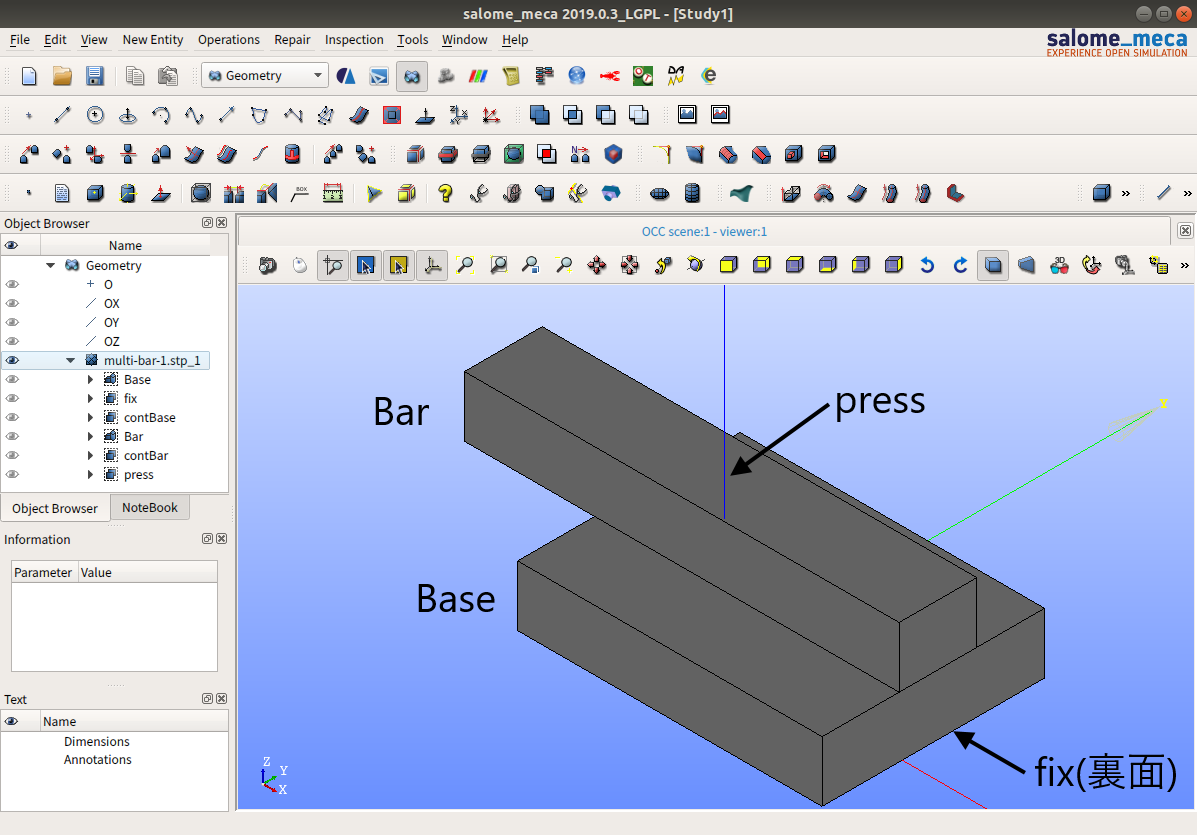
\includegraphics[width=0.9\linewidth]{fig/fig001.png}
	\end{minipage}
\end{figure}
\vspace{-\baselineskip}
\section{メッシュの作成}
連結問題と同じ方法でメッシュを切る。
ツリーは、下記。
六面体の2次メッシュとし、ジオメトリからグループを作成する。
\begin{table}[H]
	\begin{tabular}{ll}
		\quad Mesh\_1               &                  \\
		\quad *multi-bar-1.stp\_1   &                  \\
		\qquad Applied hyotheses    &                  \\
		\qquad *Automatic Length\_1 & 0.2              \\
		\qquad Applied algorithms   &                  \\
		\qquad *Regular\_1D         &                  \\
		\qquad *Quadrangle\_2D      &                  \\
		\qquad *Hexa\_3D            & 六面体のメッシュ
	\end{tabular}
\end{table}
\vspace{-\baselineskip}
\begin{figure}[H]
	%	\caption{}
	%	\label{}
	\centering
	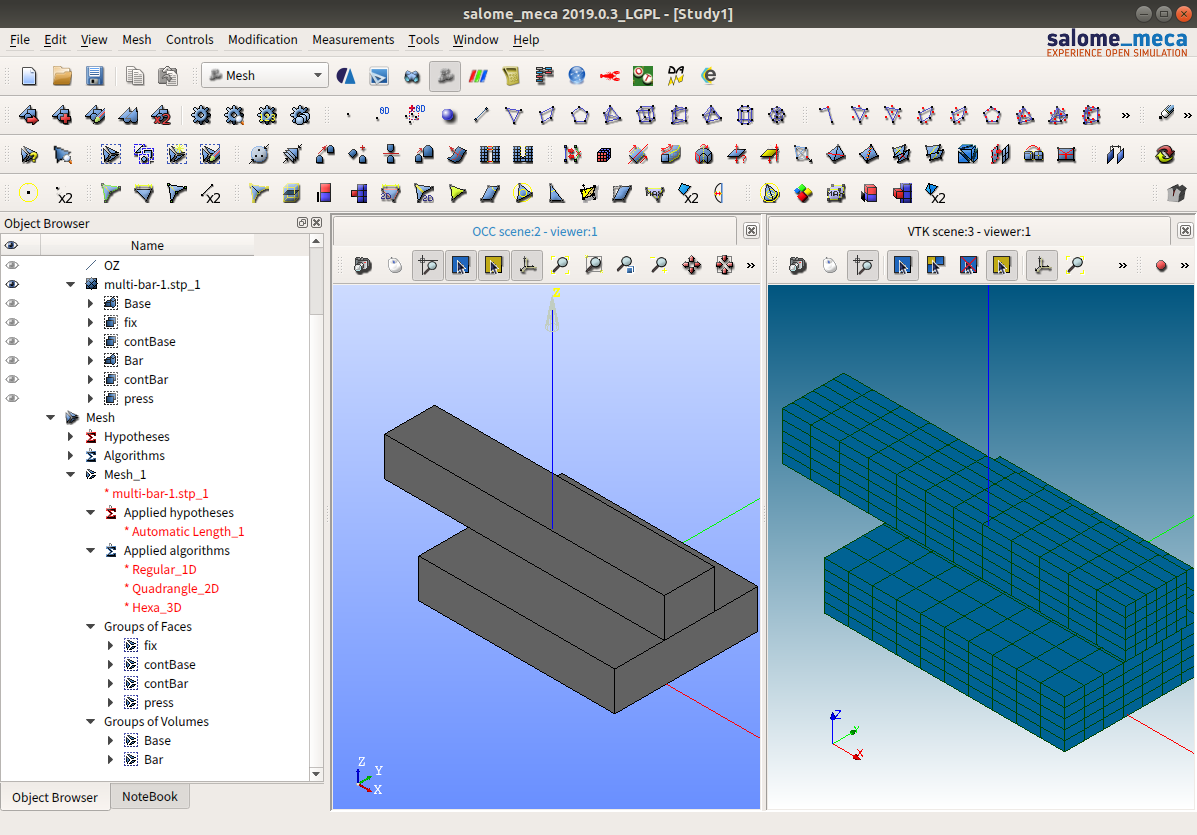
\includegraphics[width=0.9\linewidth]{fig/fig002.png}
\end{figure}
\section{解析コードの作成}
画面を\textit{AsterStudy}モジュールに変えて、アシスタント(ウィザード)を使って、通常通り\textit{Code\_Aster}の解析コードを作成する。
このとき、固定面はfix面(X=Y=Z=0)、荷重面はpress面で0.1MPaとしておく。\\
材料定数は、ベリ銅の値をそのまま使用。
\begin{itemize}
	\item ヤング率:130,300MPa
	\item ポアソン比:0.343
\end{itemize}
\textit{Code\_Aster}の結果ファイルは、フォルダー\textasciitilde/CAE/contact-bar/内に「multi-bar.rmed」として保存されるようにする。
\section{解析コードの編集}
\textit{AsterStudy}モジュールを使って、作成された解析コードを接触問題が解けるように編集する。\\
従来までの\textit{Code\_Aster}は、接触のコマンドが境界条件を設定する\textit{AFFE\_CHAR\_MECA}コマンドの下に\textit{Contact}コマンドがあったが、\textit{Salome-Meca 2010}からは、最上位に\textit{DEFI\_CONTACT}コマンドが準備されるようになった。
\subsection{境界条件の編集}
境界条件は、
\begin{enumerate}
	\item 通常の境界条件
	\item 負荷を少しづつ変化させる条件
\end{enumerate}
の2種類の条件に分けて設定する。以下に各々の境界条件設定法方について示す。
\subsubsection{通常の境界条件}
通常の境界条件は、fix面を固定する条件となる。
この境界条件は、アシスタント(ウィザード)が作成した境界条件を編集して、作成する。\\
press面をZ方向に-0.2mm変位させるが、XY方向の拘束がないので、XY方向も拘束する必要がある。
ここでXY方向を拘束(X=Y=0)する。
下記参照。
\begin{lstlisting}[caption=拘束条件,label=mecabc]
mecabc = AFFE_CHAR_MECA(DDL_IMPO=(_F(DX=0.0,
                                     DY=0.0,
                                     DZ=0.0,
                                     GROUP_MA=('fix', )),    # 固定する面(fix)を固定
                                  _F(DX=0.0,
                                     DY=0.0,
                                     GROUP_MA=('press', ))), # 負荷をかける面(press)のXY方向を固定
                        MODELE=model)
\end{lstlisting}
\subsubsection{少しづつ負荷させる境界条件作成}
press面をZ方向に-0.2mm変位させるが、この変位が接触面に直接影響を与えるので、この変位を少しづつ変化させていくようにする必要がある。
このため、この境界条件を独立させて定義する。
また、アシスタント(ウィザード)で入力した圧力の条件を削除する。
現在設定されている\textit{AFFE\_CHAR\_MECA}の後に、以下を追加する。
DZは、モデルの大きさに合わせて、設定する。
今回のモデルは、mm単位で作成されていたので、変位DZは、-0.2に設定している。
\begin{lstlisting}[caption=荷重条件,label=mecach]
mecach = AFFE_CHAR_MECA(DDL_IMPO=_F(DZ=-0.2,               # Z方向に-0.2mm変位させる
                                    GROUP_MA=('press', )), # 負荷をかける面(press)を
                        MODELE=model)
\end{lstlisting}
\subsubsection{接触の定義}
ここは、\textit{Salome-Meca 2010} で新しく設定されたコマンドになる。
従来は、境界条件(\textit{AFFE\_CHAR\_MECA})内で設定していた。
この接触の定義を\textit{DEFI\_CONTACT}で追加する、
この内容を以下で作成した。(ほとんどデフォルトのまま)
\begin{lstlisting}[caption=接触条件,label=contact]
contact = DEFI_CONTACT(FORMULATION='CONTINUE',               # 拡張ラグランジュ法(摩擦接触に対しては安定しており、推奨設定)
                       MODELE=model,
                       ZONE=_F(CONTACT_INIT='OUI',           # 接触想定領域、初期条件
                               GROUP_MA_ESCL=('contBase', ), # スレイブ面
                               GROUP_MA_MAIT=('contBar', ))) # マスター面
\end{lstlisting}
\subsection{接触の為のコード追加}
引き続き、次の行に、接触問題を解くためのコードを追加する。\\
press面の変位を0から0.2mmまで徐々に変位させていく方法を取るため、0〜0.2mmまでの中間の値をどのように設定するか(線形or非線形で回帰)を設定する。
普通に線形で回帰させる(ramp制御)方法とする。\\
このためのファンクションを下記のように定義する。\\
値は、倍率を表しており、「1」は、-0.2mmを示している。\\
座標の入力は、X,Yの形式でXYのペアで入力する。
\begin{lstlisting}[caption=増分関数,label=func]
func = DEFI_FONCTION(NOM_PARA='INST',           # 名称は任意で可。NOM_PARAは「INST(Time)」を選択。変数は、VALEで入力
                     VALE=(0.0, 0.0, 1.0, 1.0)) # 原点(0,0)から(1,1)までを線形で回帰する
\end{lstlisting}
次に1.0(1.0倍)までを何分割して解析するのかを定義する。
下記参照。
\begin{lstlisting}[caption=増分定義,label=listr]
listr = DEFI_LIST_REEL(DEBUT=0.0,                 # 初期値を設定
                       INTERVALLE=_F(JUSQU_A=1.0, # 0~1秒までを
                                     PAS=0.2))    # 0.2秒毎に5分割する。
\end{lstlisting}
\subsection{非線形解析方法の設定}
ここで今までに設定した条件、ファンクションを使って、非線形(接触)問題を解く方法を設定する。\\
アシスタント(ウィザード)で設定した\textit{MECA\_STATIQUE}は削除する。\\
\textit{Salome-Meca 2010}では、solver(\textit{STAT\_NON\_LINE})内にcontactコマンドが追加されているので、以下の様に追記した。(必要最小限の変更にした。)\\
以下のコードが\textit{STAT\_NON\_LINE}の内容。
\begin{lstlisting}[caption=非線形解析方法,label=STAT_NON_LINE]
resnonl = STAT_NON_LINE(CHAM_MATER=materfl,            # 材料を指定
                        CONTACT=contact,               # 接触を読み込む
                        EXCIT=(_F(CHARGE=mecabc),      # 通常の境界条件
                               _F(CHARGE=mecach,       # 少しづつ負荷させる条件
                                  FONC_MULT=func)),    # 中間の変位を線形で求める
                        INCREMENT=_F(LIST_INST=listr), # 0.2秒づつ増える
                        MODELE=model,                  # モデルを指定
                        NEWTON=_F(REAC_ITER=1))        # 接線剛性を更新する「ニュートン・ラプソン法」を指定
\end{lstlisting}
\subsection{Post処理の追加}
Post処理を追加する。
\textit{CALC\_CHAMP}の名前は、\textit{STAT\_NON\_LINE}で指定した名前を再利用する。
\begin{lstlisting}[caption=Post処理,label=CALC_CHAMP]
resnonl = CALC_CHAMP(reuse=resnonl,
                     CONTRAINTE=('SIGM_ELNO', 'SIGM_NOEU'), # CONTRAINTE(応力)
                     CRITERES=('SIEQ_ELNO', 'SIEQ_NOEU'),   # CRITERES(基準)
                     MODELE=model,
                     RESULTAT=resnonl)
\end{lstlisting}
\subsection{結果出力の修正}
\textit{MECA\_STATIQUE}を削除したとき、これにリンクされている結果出力側(\textit{IMPR\_RESU})がエラーになるので、この再設定が必要になる。
追加したPost処理で再設定を行う。
\begin{lstlisting}[caption=結果出力,label=IMPR_RESU]
IMPR_RESU(FORMAT='MED',              # 出力するバイナリ形式にMED形式を指定
          RESU=_F(NOM_CHAM=('DEPL', 'SIEQ_NOEU', 'SIGM_NOEU'), # DEPL(変位量)、SIEQ_NOEU(等価応力(節点))、SIGM_NOEU(応力(節点))
                  RESULTAT=resnonl), # 論理ユニット番号
          UNITE=80)
\end{lstlisting}
\section{解析の開始}
通常通り、解析をスタートさせる。
% 警告はでるが、エラーなく終了。
\section{計算結果の確認}
計算が終了したので、結果を確認する。
以下が確認した結果になる。
うまく計算できている。
\begin{figure}[H]
	%	\caption{}
	%	\label{}
	\centering
	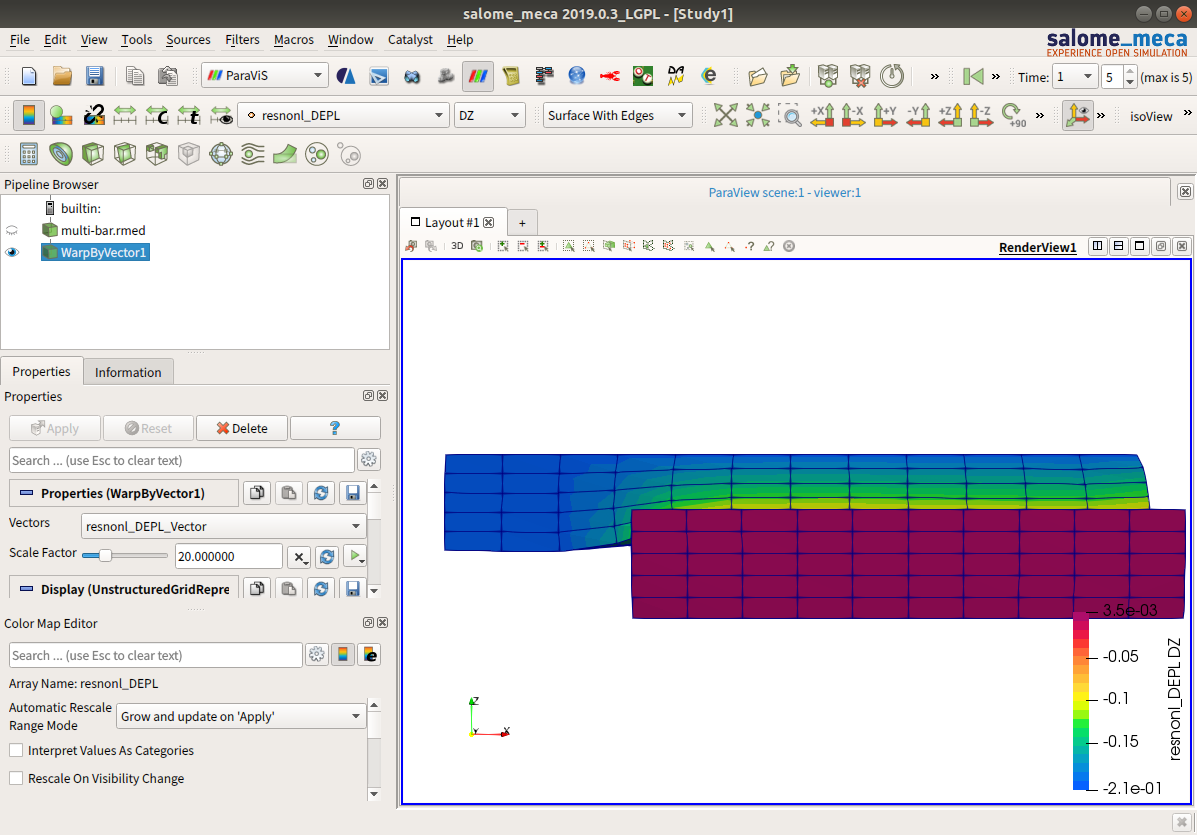
\includegraphics[width=0.9\linewidth]{fig/fig003.png}
\end{figure}
\section{接触面積が増加するモデルの場合}
前記のモデルは、接触するものが四角柱のため、変形しても接触面積は変化しない。
このため、接触面のエッジにR面取りを施し、変形と共に接触面積が増加するモデルを作って解析してみる。
\subsection{モデルの読み込み}
モデルは、「multi-bar-1-R.stp」を読み込む。
接触面のエッジをR面取りしたモデル。
解析は、\textasciitilde /CAE/contacr-R/のフォルダーを作り、この中で解析する。
\subsection{Entityの作成}
グループ化は、まったく同じように実施。
ただし、Barの接触面(contBar)は、接触する平面と変形と共にR面にも接触することになるので、平面+R面をcontBarとしている。
\begin{figure}[H]
	\begin{minipage}{0.34\hsize}
		\begin{table}[H]
			\centering
			\begin{tabular}{@{}ll@{}}
				\toprule
				グループ名 & 備考             \\\midrule
				Base       & Solid1(Base)     \\
				fix        & 固定面           \\
				contBase   & Baseの接触面     \\
				Bar        & Solid2(Bar)      \\
				contBar    & Barの接触面      \\
				press      & 荷重を負荷する面 \\\bottomrule
			\end{tabular}
		\end{table}
	\end{minipage}
	%
	\begin{minipage}{0.64\hsize}
		%	\caption{}
		%	\label{}
		\centering
		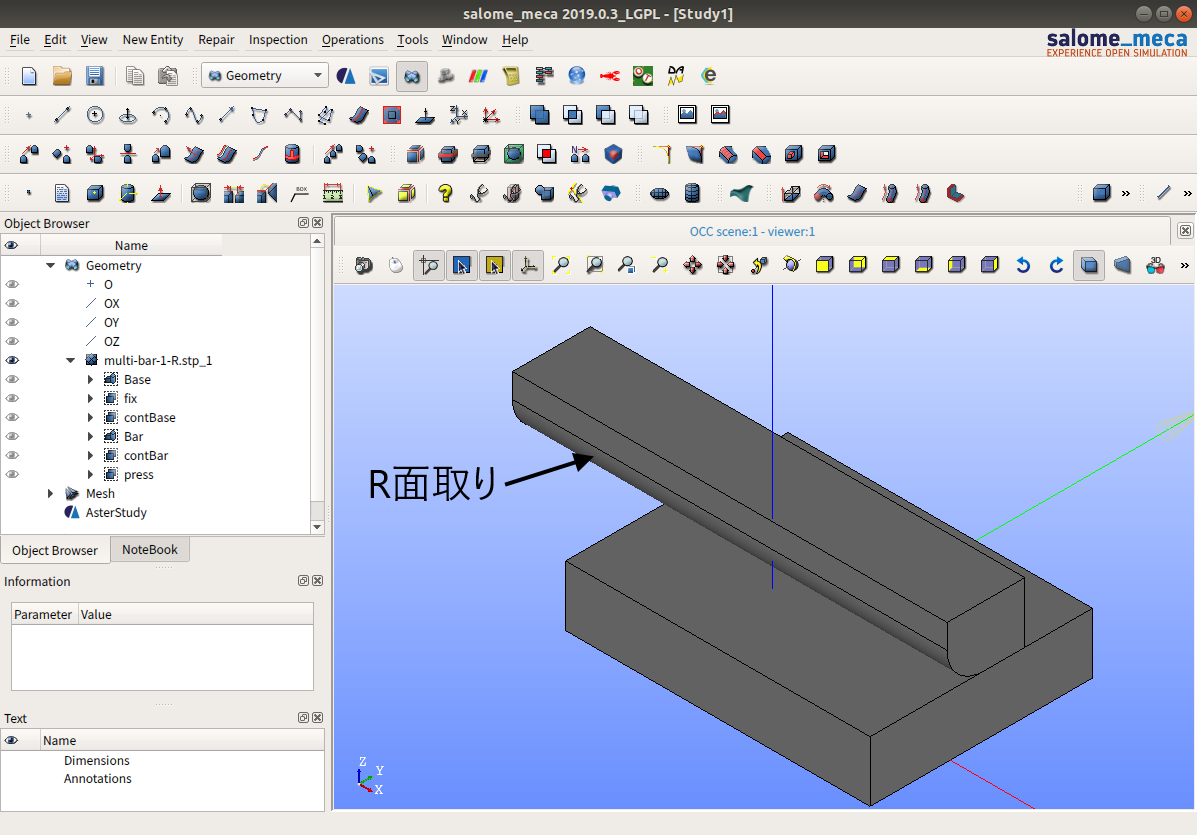
\includegraphics[width=0.9\linewidth]{fig/fig004.png}
	\end{minipage}
\end{figure}
\subsection{メッシュの作成}
メッシュは、六面体だと、エラーが発生し、メッシュが切れなかったので、四面体の2次メッシュとし、Automatic Length=0.2とした。
次図参照。
\begin{figure}[H]
	%	\caption{}
	%	\label{}
	\centering
	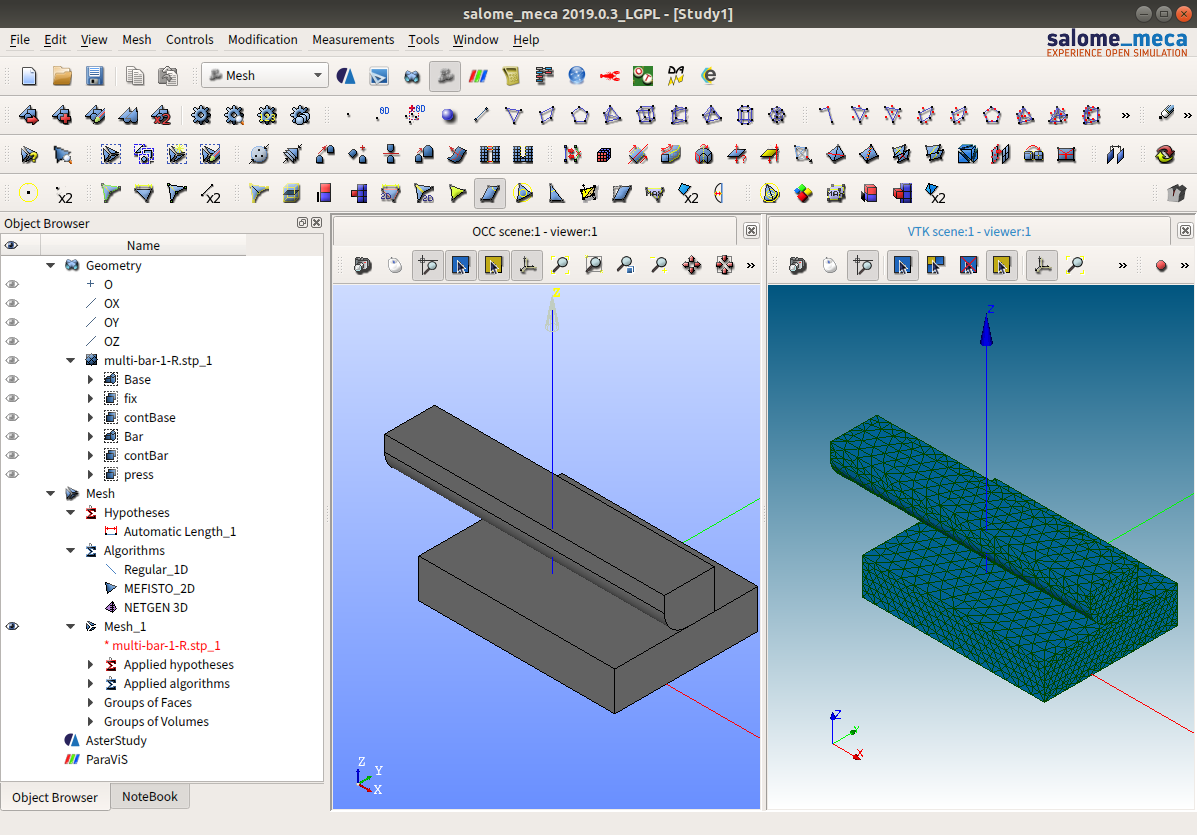
\includegraphics[width=0.9\linewidth]{fig/fig005.png}
\end{figure}
\subsection{解析コードの作成}
同じ方法で作成。
\subsection{解析開始}
% 計算開始させると0.2から0.4までは、時間が掛かる(約20分)ものの、うまく収束していたが、0.6から収束しなくなり、Itaration No.が15を超えてしまう。
% それまでは、多くても5回で収束していた。
% R付けしている為、収束し難いと思い、INTERVALLEのPASを0.1に変更し、0.1毎に計算させるように変更したが、約40分たっても答えが出ない。
% (途中で計算をキャンセル)
% Projectionを2次に変えても、Methodを変えても同じ結果。
% この為、メッシュを2次メッシュから1次メッシュに変更して、再トライした。
% この結果、計算時間は、144秒(CPU時間75秒)で計算が終了。驚くほど計算が早い。
% 「2次メッシュは収束し難い。非線形の場合、メッシュは1次メッシュで細かいメッシュにする。」と言う事は事実だった。
% 上記内容は、Salome-MECA-2007.1の場合であり、2008.1では、確認していない。
通常通り、解析をスタートさせる。
エラーが発生し、解析が終了する。\\
メッセージファイルを確認すると、ニュートン法の最大繰り返し回数で収束しなかったために停止している。\\
ニュートン法の最大繰り返し回数を増やして再計算を実行する。
\begin{lstlisting}[caption=非線形解析を修正,label=STAT_NON_LINE2]
resnonl = STAT_NON_LINE(CHAM_MATER=materfl,
                        CONTACT=contact,
                        CONVERGENCE=_F(ITER_GLOB_MAXI=30), # ニュートン法の最大繰り返し回数を追加(デフォルト値は10)
                        EXCIT=(_F(CHARGE=mecabc),
                               _F(CHARGE=mecach,
                                  FONC_MULT=func)),
                        INCREMENT=_F(LIST_INST=listr),
                        MODELE=model,
                        NEWTON=_F(REAC_ITER=1))
\end{lstlisting}
\subsection{結果の確認}
最大応力は、3,400MPaでRの根元部で発生。
% Rの為、食い込みが少ないので、応力が下がる?
変形の様子を確認すると、R面に沿ってBase側が変形していることがわかる。
(変形と共に接触面積が増える。
$\rightarrow$
非線型になっている。)
\begin{figure}[H]
	\begin{minipage}{0.49\hsize}
		\captionsetup{labelformat=empty,labelsep=none}
		\caption{変位}
		%	\label{}
		\centering
		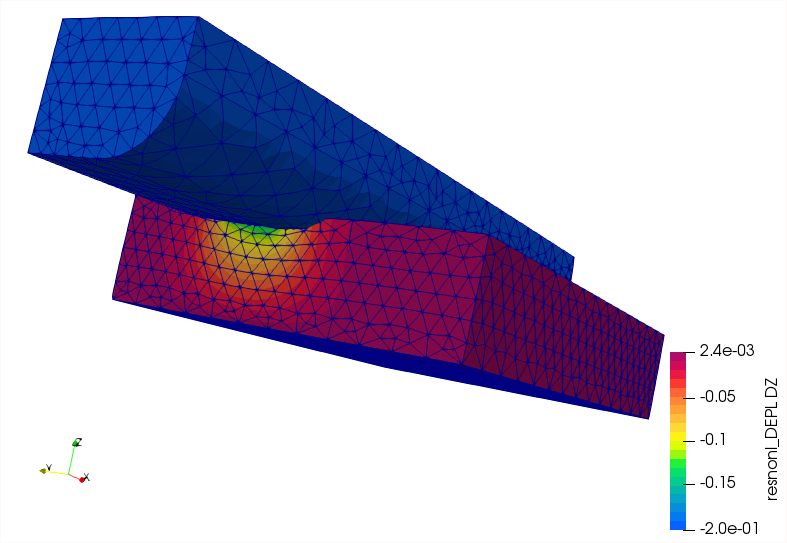
\includegraphics[width=0.9\linewidth]{fig/fig006.png}
	\end{minipage}
	\begin{minipage}{0.49\hsize}
		\captionsetup{labelformat=empty,labelsep=none}
		\caption{相当応力}
		%	\label{}
		\centering
		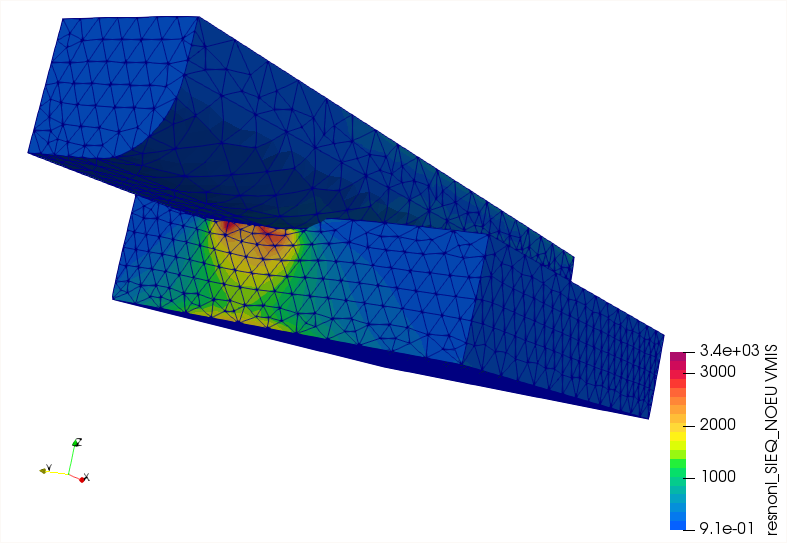
\includegraphics[width=0.9\linewidth]{fig/fig007.png}
	\end{minipage}
\end{figure}
\section{接触面積が減少するモデルの場合}
変形と共に接触面積が減少していくモデルを考える。
下記のように変形と共にPlateの両端が持ち上がり、接触面積が減少していく場合を考える。\\
下記モデルで解析し、Plateの両端が持ち上がっている(接触面積が減少する)かどうかを確認する。
\subsection{モデルの読み込み}
モデルは、「test-contact-1.stp」を読み込む\footnote{モデルを読み込むと、モデルの上下方向がY軸方向となっているので、\menu[,]{Operations,Transformation,Rotation}で、OX軸に対して90度回転させている。}。\textasciitilde /CAE/contact-plate/というフォルダーを作りこの中で解析する。
\subsection{Entityの作成}
基本的には、前記したモデルと同じ。
違いは、contBaseが2ヶ所ある(2平面をグループ化してcontBaseとした)ことと、press面はPlate中央の円柱の上面としていること。
\begin{figure}[H]
	\begin{minipage}{0.34\hsize}
		\begin{table}[H]
			\centering
			\begin{tabular}{@{}ll@{}}
				\toprule
				グループ名 & 備考             \\\midrule
				Base       & Solid1(Base)     \\
				fix        & 固定面           \\
				contBase   & Baseの接触面     \\
				Plate      & Solid2(Plate)    \\
				contPL     & Plateの接触面    \\
				press      & 荷重を負荷する面 \\\bottomrule
			\end{tabular}
		\end{table}
	\end{minipage}
	%
	\begin{minipage}{0.64\hsize}
		%	\caption{}
		%	\label{}
		\centering
		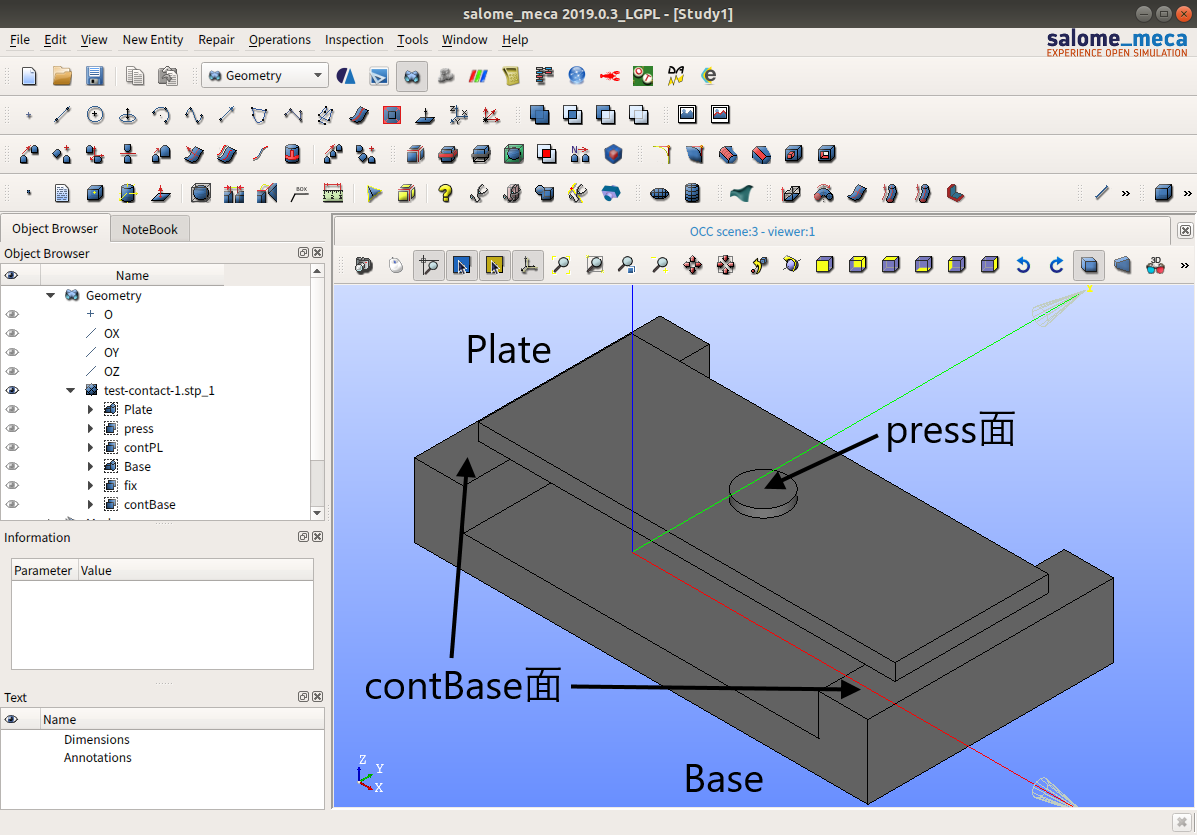
\includegraphics[width=0.9\linewidth]{fig/fig008.png}
	\end{minipage}
\end{figure}
\subsection{メッシュの作成}
四面体の2次メッシュとした。
細かさは、AutomaticLength=0.1。
% (2次メッシュにはしていない。)
\\形状が複雑な分、メッシュが細かい。
\begin{figure}[H]
	%	\caption{}
	%	\label{}
	\centering
	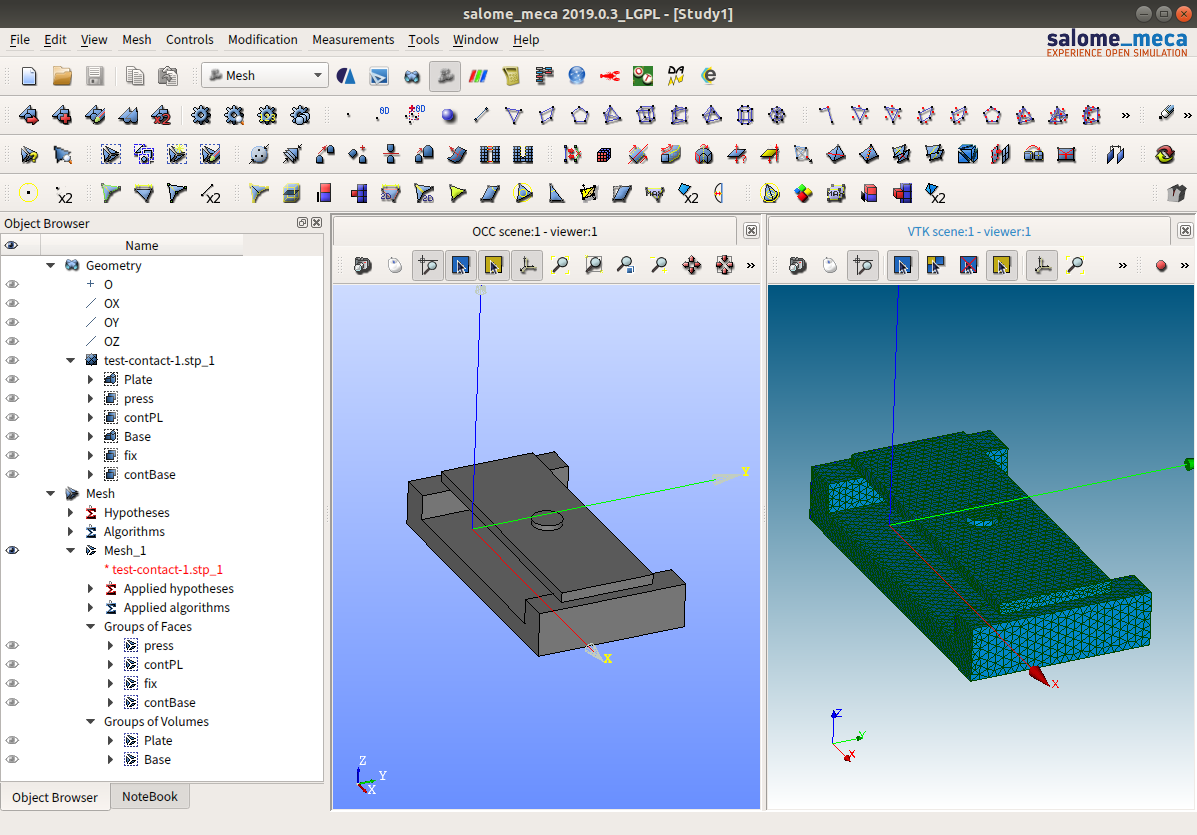
\includegraphics[width=0.9\linewidth]{fig/fig009.png}
\end{figure}
\subsection{解析コードの作成}
コード自体は、ほとんど同じ。
press面の変位は、持ち上がりが確認できるように、大きな値(Y方向に-0.5mm)に設定。
\subsection{計算}
形状が複雑な分メッシュが多くなってしまっているので、計算時間は、長くかかる。
% 875秒(約15分)、CPU時間474秒であり、長く掛かった。
% ←Salome-MECA-2007.1の場合。
% 2008.1の場合は、186秒(約6分)、CPU時間212秒であり、約2倍の速さに変わっている。
変位の結果を確認すると、Plateの両端が持ち上がっているのが確認できる。
(下図参照。)
正しく接触判定をして、計算している。
\begin{figure}[H]
	\begin{minipage}{0.49\hsize}
		\captionsetup{labelformat=empty,labelsep=none}
		\caption{変位(倍率5倍で表示)}
		%	\label{}
		\centering
		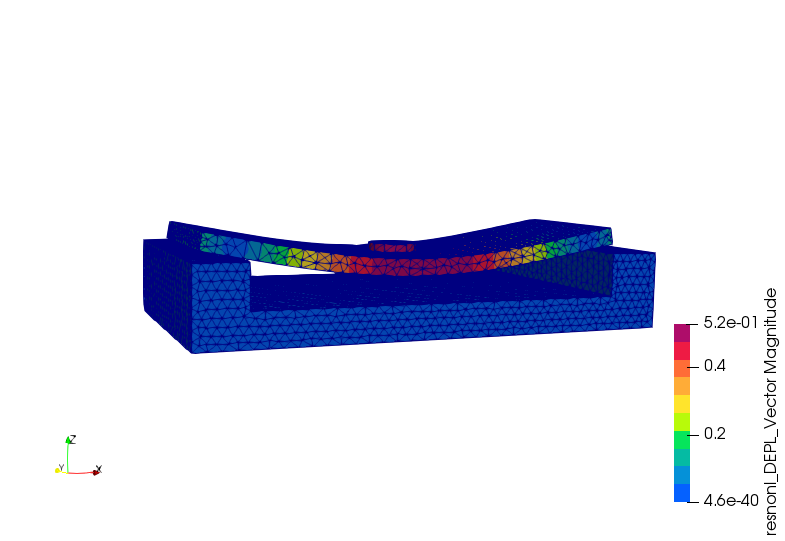
\includegraphics[width=0.9\linewidth]{fig/fig010.png}
	\end{minipage}
	\begin{minipage}{0.49\hsize}
		\captionsetup{labelformat=empty,labelsep=none}
		\caption{拡大}
		%	\label{}
		\centering
		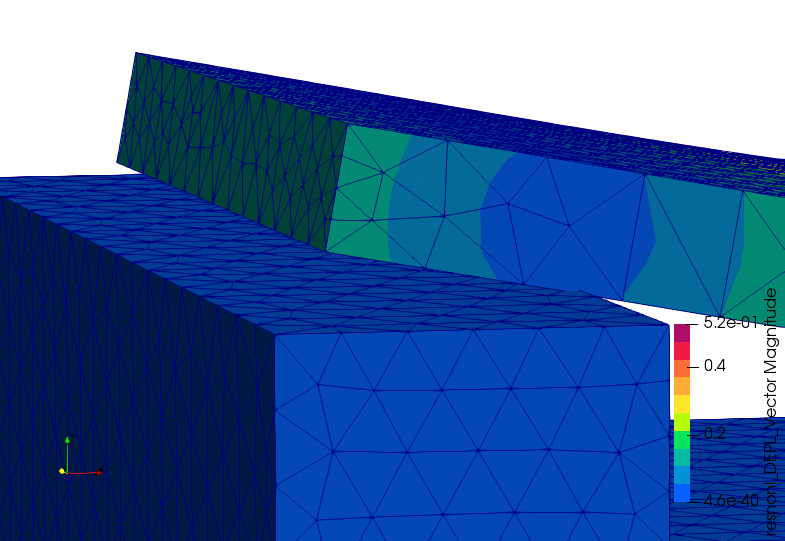
\includegraphics[width=0.9\linewidth]{fig/fig011.png}
	\end{minipage}
\end{figure}
\section{ソースコード}
\lstinputlisting[caption=multi-bar.commの場合,label=multi-bar]{fig/multi-bar.comm}
\lstinputlisting[caption=multi-bar-R.commの場合,label=multi-bar-R]{fig/multi-bar-R.comm}
\lstinputlisting[caption=contact-plate.comm(R面取りしたモデル)場合,label=contact-plate]{fig/contact-plate.comm}
\end{document}